\documentclass[handout]{beamer}
\usetheme{CambridgeUS} % replace it with Boadilla if you want no section bar
%\usecolortheme{crane} % other ones: dove, dolphin, rose, seahorse, orchid, crane, seagull, lily, wolverine
%\usefonttheme{serif} 
\usefonttheme[onlymath]{serif} % uncomment if you want it just for math

\setbeamertemplate{navigation symbols}{}  % comment to have nagivation

\usepackage[compress,comma,authoryear]{natbib}
\usepackage{tikz}
\usetikzlibrary{mindmap,trees}
\usepackage{amsmath,mathtools}
\usepackage{amsthm}
\usepackage{booktabs}
\usepackage{graphicx,epstopdf}
\usepackage{hyperref}


\definecolor{blue}{RGB}{0,114,178}
\definecolor{orange}{RGB}{213,94,0}
\definecolor{red}{RGB}{190,0,0}
\definecolor{yellow}{RGB}{240,228,66}
\definecolor{green}{RGB}{0,158,115}
\definecolor{Lblue}{RGB}{0,197,155}
\definecolor{Dblue}{RGB}{0,76,119}
\definecolor{Lgreen}{RGB}{180,255,230}

\hypersetup{
	colorlinks=false,
	linkbordercolor = {white},
	linkcolor = {blue}
}
\definecolor{MyBackground}{RGB}{245,245,245}

\setbeamercolor{frametitle}{fg=blue}
\setbeamercolor{title}{fg=blue}
\setbeamertemplate{footline}[frame number]
\setbeamertemplate{navigation symbols}{} 
\setbeamertemplate{itemize item}[circle]%{$\bigstar$}
\setbeamertemplate{itemize subitem}{$\bigstar$}
\setbeamercolor{itemize item}{fg=blue}
\setbeamercolor{itemize subitem}{fg=blue}
\setbeamercolor{enumerate item}{fg=blue}
\setbeamercolor{enumerate subitem}{fg=blue}
\setbeamercolor{button}{bg=MyBackground,fg=blue}
\setbeamercolor*{palette primary}{use=structure,fg=blue,bg=white}
\setbeamercolor*{palette secondary}{use=structure,fg=white,bg=Dblue}
\setbeamercolor*{palette tertiary}{use=structure,fg=white,bg=blue}
\setbeamercolor*{palette quaternary}{fg=white,bg=black}
\setbeamercolor*{palettes quaternary}{fg=white,bg=Lgreen}
%\setbeamercolor{titlelike}{parent=structure,bg=Lgreen}
%\setbeamercolor{title in head/foot}{bg=Lgreen,fg=orange}

\setbeamertemplate{enumerate item}{%
	\usebeamercolor[bg]{item projected}%
	\raisebox{1.5pt}{\colorbox{blue}{\color{fg}\footnotesize\insertenumlabel}}%
}



\begin{document}
	\title[Econometrics 2]{Econometrics 2 (M.Sc.)}
	\subtitle{Regression and Causality}
	\author[Mohammad Hoseini]{Mohammad Hoseini}
	
	%\institute[IMPS]{Institute for Management and Planning Studies (IMPS)}
	
	\date[Spring 2024]{Spring 2024 \\
	\vspace{10pt} @metrics2
}
	
\begin{frame}[plain]
	\titlepage
\end{frame}


\section{Regression and Causality}

\begin{frame}{Overview}
In the previous lecture, we discussed how selection bias can distort observed effect from the causal treatment effect.\bigskip

We saw how randomization can remove selection bias.\bigskip

In this lecture, we talk over another basic method to remove selection bias which is called ``conditional independence assumption'' (CIA).\bigskip

In simple words, this method relies on adding ``proper'' control variables to the OLS for removing selection bias.
\end{frame}

\begin{frame}{Overt and covert selection biases}
\textbf{Overt bias}: selection bias due to observables $X$\medskip

If selection bias is only due to overt bias: 
\[Y^D\perp D \text{ may not hold but } Y^D\perp D | X \text{ holds.}\] 
\[E(Y^D_i| D)=E(Y^D_i) \text{ may not hold but } E(Y^D_i| D_i,X_i)=E(Y_i^D|X_i) \text{ holds.}\] This situation is called \textbf{selection-on-observables}.\bigskip\pause

\textbf{Covert (hidden) bias}: selection bias due to unobservables $\varepsilon$\medskip

If selection bias is due to hidden bias:
\[Y^D\perp D|X \text{ may not hold but } Y^D\perp D | (X,\varepsilon) \text{ holds.}\]This situation is called \textbf{selection-on-unobservables}.\medskip

We can remove overt bias by controlling for $X$, but hidden bias is tricky. 
\end{frame}


\begin{frame}{Selection biases in linear models}
Suppose the true potential response model is linear such that $Y_i^d=\beta_d+\gamma_d X_i+\varepsilon_i^d$
and

$\qquad\qquad Y_i^1-Y_i^0=\beta_1-\beta_0+(\gamma_1-\gamma_0)X_i+\varepsilon_i^1-\varepsilon_i^0 $\pause

Treatment effect: $E[Y_i^1-Y_i^0]=\beta_1-\beta_0+(\gamma_1-\gamma_0)E[X] $\medskip\pause

Observed effect if a selection bias exist such that $D_i=\begin{cases}
1,&Y_i^1>Y_i^0\\ 0, & Y_i^1<Y_i^0
\end{cases}$:
\begin{align*}
E[&Y|D=1]-E[Y|D=0]&\\
=&{\scriptstyle \beta_1-\beta_0+\gamma_1E[X|D=1]-\gamma_0E[X|D=0]+ E[\varepsilon^1|D=1]-E[\varepsilon^0|D=0]}&\\
= & \ \beta_1-\beta_0+(\gamma_1-\gamma_0)E[X]&\text{(treatment)}\\
+ & \gamma_1(E[X|D=1]-E[X])-\gamma_0(E[X|D=0]-E[X]) &\text{(overt bias)}\\
+ & E[\varepsilon^1|D=1]-E[\varepsilon^0|D=0] &\text{(hidden bias)}
\end{align*}\pause
If $E(X|D)=E[X]$ over bias disappears.

If $E[\varepsilon^1|D=1]=E[\varepsilon^0|D=0]$ hidden bias disappears.
\end{frame}

\begin{frame}{Conditional Independence Assumption (CIA)}
\textbf{Selection-on-observables:} Conditional on observable characteristics $X_i$, treatment $D$ is as good as random assignment.
%X is the only reason that $\eta_i$ and $D_i$ are correlated in $Y_i = \alpha+\beta D_i+\eta_i$.
\[Y_i^D\text{ is independent of }D_i, \text{ conditional on } X_i\]
\[E[Y_i^1|X_i,D_i=1]=E[Y_i^1|X_i,D_i=0]=E[Y_i^1|X_i] \]
\[E[Y_i^0|X_i,D_i=1]=E[Y_i^0|X_i,D_i=0]=E[Y_i^0|X_i] \]
If we are looking at individuals with the same characteristics $X$, then the potential outcomes $Y^D_i$ and $D_i$ are independent. \medskip

Given CIA, conditional-on-$X_i$ comparison of average outcome between treatment and control groups has a causal interpretation:
\[E[Y_i^1|X_i,D_i = 1] - E [Y_i^0|X_i,D_i = 0] = E [Y_i^1- Y_i^0|X_i]\]

\end{frame}


\begin{frame}{When selection-on-observable goes wrong}
	Effect of winning the Oscars on an actor's income
	\begin{table}
		\begin{tabular}{|l|c|c|}
			\hline
			Observable variables in data& Person 1 & Person 2 \\
			\hline
			%occupation & actor & actor \\
			birth year & 1974 & 1974\\
			gender & male & male \\
			marital status & married & married \\
			children & 1&1\\
			sample work & Joker & Joker \pause\\
			\hline
			&&\\
			\begin{minipage}{.4\linewidth}
				{\color{red}	including unobservables:\vspace*{1.5cm} }
			\end{minipage}
			&	\includegraphics[width=0.15\linewidth]{./Figures/Phoniex2.png}&	\includegraphics[width=0.15\linewidth]{./Figures/ghafourian.jpg} \\
			&Joaquin Phoenix & Mehran Ghafourian \\
			\hline
		\end{tabular}
	\end{table}
	
\end{frame}

\begin{frame}{CIA and regression estimation}
One way to estimate causal effect with CIA is using regression, but it implicitly assumes that $Y_i^D$ is both linear in $D$ and the same for everyone except for an additive error term.\medskip

$ Y_i= \alpha+\beta D_i+\eta_i, \quad E[D_i\eta_i]\neq0$ (which means $E[\eta_i|D_i=1]\neq0$)\medskip
\pause

If CIA holds only overt bias exist and given a vector of observed variable, $X_i$, we can decompose $\eta_i$ into \vspace{-5pt}
\[\eta_i=\gamma X_i+v_i, \ \text{ where  } \ E[\eta_i|X_i]=\gamma X_i,   \ E[v_i]=0, \ E[D_iv_i]=0 \]\pause
Then in linear model $ Y_i= \alpha+\beta D_i+\gamma X_i+v_i$, $v_i$ is uncorrelated with $D_i$ and $X_i$, and $\beta$ is the causal effect of interest. %To see why note that 
%\[ E[Y^1_i|D_i=1,X_i]= \alpha+\beta+\gamma X_i, \ \ E[Y^0_i|D_i=0,X_i]= \alpha+\gamma X_i\]
In fact, the conditional treatment effect under CIA is: 
\[ E[Y_i^1-Y_i^0|X_i]=\beta+\gamma X_i\]

\end{frame}


\begin{frame}{Multinomial treatment}
Instead of (treatment, no treatment), we have (treatment 1, treatment 2, treatment 3, \dots)\bigskip

We can generalize the previous results:
\[Y^S_{i}\equiv f_i(S) , \quad S=1,\dots,n \]
Selection bias disappears when \[E[Y^S_{i}|S=s_i]=E[Y^S_{i}|S=s_j], \ i\neq j \]
If the people who are in state $s_j$, had been in state $s_i$, they would have the same expected outcome as people who are in state $s_i$.\medskip

CIA: $\qquad E[Y^S_{i}|X_i,S=s_i]=E[Y^S_{i}|X_i,S=s_j], \ i\neq j$

\end{frame}

\begin{frame}{Years of schooling and wage}
$Y^S_i:$ Potential wage associated with schooling level $S$ for individual $i$.\bigskip

CIA: conditional on $X_i$, $Y^S_i$ is independent of $S_i$, and the average causal effect of a one-year increase in schooling is
$E(Y_i^S-Y_i^{S-1}|X_i)$\bigskip

Assume that $Y_i^S=\alpha+\beta S +\zeta_i$. 
In terms of observables: $Y_i=\alpha+\beta s_i+\eta_i$.\bigskip

If CIA holds given a vector of observed covariates $\eta_i=\gamma X_i+v_i$, and $E (Y_i^S|X_i, s_i) = E (Y_i^S|X_i)=\alpha+\beta S+\gamma X_i$. Then:\bigskip

\[E[Y_i^S-Y_i^{S-1}|X_i] = \beta + \gamma X_i\]
%The regression coefficient $\beta$ is the causal effect of interest and can be interpreted as an average of the individual specific difference $Y_i^S-Y_i^{S-1}|X_i$.\medskip

%How to find $Y_i^S-Y_i^{S-1}$? \pause we can do something by matching that we talk later.
\end{frame}

\begin{frame}{What variables to control?}
Assume we want to estimate a causal relationship using CIA.\bigskip

An important point is what variables should be controlled for?\bigskip

The general rule is that we should only control for variables that make CIA more plausible.\bigskip

Two criterion to consider
\begin{itemize}
\item Omitted variable bias
\item Bad controls problem
\end{itemize}\medskip

In simple terms: control for pretreatment covariates, but not control for variables that are themselves outcome variables.\medskip

In the following, we discuss them in five cases.
\end{frame}

\begin{frame}{Practical cases where controlling is allowed or not}
%The arrows mean  causing or affecting\bigskip

\begin{tabular}{|l|l|c|}\hline
Case 1 & X must be controlled.&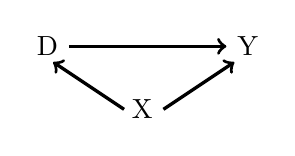
\begin{tikzpicture}
\draw[->,very thick] node [left] {D} (0,0)  -- (2,0) node [right] {Y} ;
\draw[->,very thick]  (1.2,-.8) node [left] {X}  -- (2.1,-.2) ;
\draw[->,very thick] (.7,-.8) -- (-.2,-.2)  ;
\end{tikzpicture}\\
\hline
Case 2 & No need to control for X &
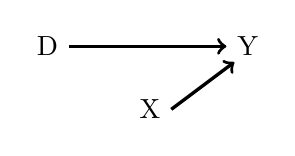
\begin{tikzpicture}
\draw[->,very thick] node [left] {D} (0,0)  -- (2,0) node [right] {Y} ;
\draw[->,very thick]  (1.3,-.8) node [left] {X}  -- (2.1,-.2) ;
\end{tikzpicture} \\
\hline
Case 3 & Not control for Z & 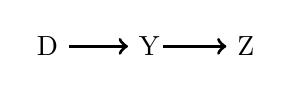
\begin{tikzpicture}
\draw[->,very thick] node [left] {D} (0,0)  -- (0.75,0) node [right] {Y} ;
\draw[->,very thick]  (1.2,0) -- (2,0)  node [right] {Z}  ;
\end{tikzpicture} \\
\hline
Case 4 & Not control for W for total effect&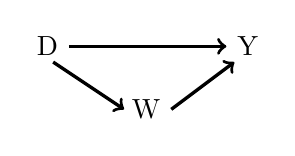
\begin{tikzpicture}
\draw[->,very thick] node [left] {D} (0,0)  -- (2,0) node [right] {Y} ;
\draw[->,very thick]  (1.3,-.8) node [left] {W}  -- (2.1,-.2) ;
\draw[<-,very thick] (.7,-.8) -- (-.2,-.2)  ;
\end{tikzpicture}\\
\hline
Case 5 & Proxy variable $X_p$ &
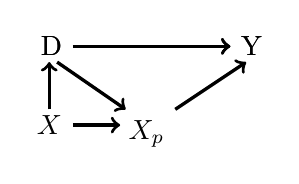
\begin{tikzpicture}
\draw[->,very thick] node [left] {D} (0,0)  -- (2,0) node [right] {Y} ;
\draw[->,very thick] node [left] {D} (0,0)  -- (2,0) node [right] {Y} ;
\draw[->,very thick]  (1.3,-.8) node [below left] {$X_p$}  -- (2.2,-.2) ;
\draw[<-,very thick] (.67,-.8) -- (-.2,-.2)  ;
\draw[->,very thick]  (0,-1) node [left] {$X$}  -- (.6,-1) ;	\draw[->,very thick]  (-.3,-.8)  -- (-.3,-0.2) ;	
\end{tikzpicture}\\ \hline	

\end{tabular}

\end{frame}

\begin{frame}{Case 1: $X$ must be controlled for}
\begin{center}
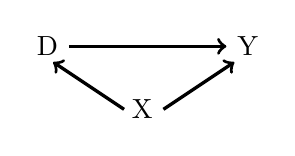
\begin{tikzpicture}
\draw[->,very thick] node [left] {D} (0,0)  -- (2,0) node [right] {Y} ;
\draw[->,very thick]  (1.2,-.8) node [left] {X}  -- (2.1,-.2) ;
\draw[->,very thick] (.7,-.8) -- (-.2,-.2)  ;
\end{tikzpicture}
\end{center}
Here $X$ is a \textit{common factor} and we must control for it, otherwise we encounter Omitted Variable Bias (OVB) problem.\medskip

$X$ is also called ``confounder''. If there is no causal relationship from $D$ to $Y$ (the arrow between $D$ and $Y$ is removed), we still see a correlation between them because of common factor $X$.\bigskip

Ex: $X$ health status, $D$ working, $Y$ doctor visit
\[Y_i=\alpha+\beta D_i+e_i \qquad Y_i=\alpha'+\beta' D_i+\gamma X_i+e'_i  \]
$\beta$ negative and significant (bad model), $\beta'$ insignificant (good model).

\end{frame}

\begin{frame}{Omitted variable bias}
Suppose we want to estimate schooling regression, and schooling ($D_i$) and ability ($X_i$) are the determinants of wage ($Y_i$):\medskip

Long regression: $Y_i=\alpha+\beta D_i+\gamma X_i +\epsilon_i$\medskip

Short regression: $Y_i=\alpha'+\beta' D_i+\epsilon'_i$\bigskip

If $X_i$ and $D_i$ are correlated ($D_i$ is not necessarily the cause of $X_i$): 
\[X_i=\delta_0+\delta D_i + e_i \ \Rightarrow \ Y_i=\alpha+\gamma\delta_0+(\beta+\gamma\delta)D_i+(\epsilon_i+\gamma e_i) \]
$\beta'=\beta+\gamma\delta$ is biased. 
\medskip

When OVB is not present?\pause
\begin{itemize}
\item $\gamma=0 \rightarrow X_i$ is not omitted (uncorrelated with $Y_i$)
\item $\delta=0 \rightarrow X_i$ is uncorrelated with $D_i$
\end{itemize}

\end{frame}


\begin{frame}{Case 2: no need to control for X}
\begin{center}
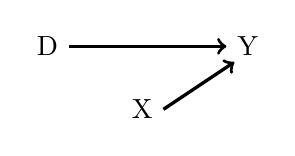
\begin{tikzpicture}
\draw[->,very thick] node [left] {D} (0,0)  -- (2,0) node [right] {Y} ;
\draw[->,very thick]  (1.2,-.8) node [left] {X}  -- (2.1,-.2) ;
\end{tikzpicture}
\end{center}
When $X$ and $D$ are uncorrelated ($\delta=0$ in the previous slide), no arrow between $D$ and $X$ exists and controlling for $X$ does not matter.\medskip

In randomized experiments, $D$ is random and no common factor or confounder $X$ create problem. \bigskip

Randomization solves omitted variable problem.\medskip

In randomized/natural experiments, no worries for OVB.

\end{frame}
%
%\begin{frame}{CIA and natural experiments}
%Previously, we talked about using natural/quasi experiments.\medskip
%
%What if the experiment is ``unnatural''?\medskip
%
%For instance, suppose that we have state-level data and $D$ is decided by each state's economic, demographic, and political variables reflected in vector $X$.\medskip
%
%These variables might also influence the individual outcome.\medskip
%
%In such a case, the state-level covariate $X$ should be controlled for to ensure that $Y^d\perp D|X$, otherwise there is a omitted variable bias.
%
%\[ Y_i= \alpha+\beta D_i+X_i'\gamma+v_i\]
%\end{frame}

\begin{frame}{Case 3: Not control for Z}
\begin{center}
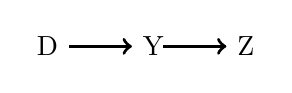
\begin{tikzpicture}
\draw[->,very thick] node [left] {D} (0,0)  -- (0.8,0) node [right] {Y} ;
\draw[->,very thick]  (1.2,0) -- (2,0)  node [right] {Z}  ;
\end{tikzpicture}
\end{center}

When $Z$ is a post response variable, it should not be controlled because fixing $Z$ in this case will remove part or all effect of $D$ on $Y$.\medskip

At the extreme, if $Z$ is a function of $Y$ then fixing $Z$ is the same as fixing $Y$, which results in zero treatment effect.\medskip

Example: $D$ education in a year, $Y$ is GPA, $Z$ is college entrance next year.
\end{frame}

\begin{frame}{Example}
	\begin{center}
		\includegraphics[width=.9\textwidth]{./Figures/2-ovb.png}
	\end{center}
\end{frame}

\begin{frame}{Case 4: Not control for $W$ to estimate overall effect}
\begin{center}
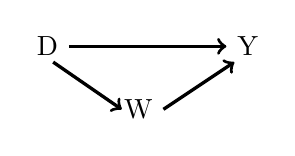
\begin{tikzpicture}
\draw[->,very thick] node [left] {D} (0,0)  -- (2,0) node [right] {Y} ;
\draw[->,very thick]  (1.2,-.8) node [left] {W}  -- (2.1,-.2) ;
\draw[<-,very thick] (.67,-.8) -- (-.2,-.2)  ;
\end{tikzpicture}\qquad
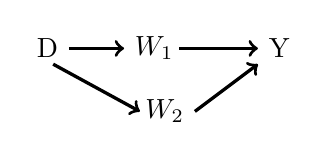
\begin{tikzpicture}
\draw[->,very thick] node [left] {D} (0,0)  -- (.7,0) node [right] {$W_1$};
\draw[->,very thick]  (1.4,0) -- (2.4,0) node [right] {Y} ;
\draw[->,very thick]  (1.6,-.8) node [left] {$W_2$}  -- (2.4,-.2) ;
\draw[<-,very thick] (.9,-.8) -- (-.2,-.2)  ;
\end{tikzpicture}
\end{center}
When $D$ affects $Y$ through multiple routes ($W_1,W_2,\dots$), to estimate the total effect of $D$ on $Y$, controlling for $W_i$ is not allowed.\medskip 

BUT if we want to know the effect of $D$ on $Y$ ``net of $W$'', then controlling for $W$ is fine.\medskip

Example: $D$ schooling, $Y$ wage, $W$ getting the diploma.\medskip

What is the spillover gains of schooling rather than getting the diploma? 
\end{frame}


\begin{frame}{Bad controls}
Case 3 and 4 (for overall effect) are the examples of \textbf{bad control} problem.\medskip

Bad controls are variables that are themselves outcome and like dependent variables.\medskip

Good controls are exogenous variables and can think of having been fixed at the time of experiment.\bigskip\pause

Example: suppose we are interested in  the effects of a college degree on earnings and there are two types of jobs - white collar (higher-paying) and blue collar (lower-paying). \medskip


Is occupation like an omitted variable in schooling regression?

Why might this not be a good idea to add controls of occupation in the regression?
\end{frame}

\begin{frame}{Bad controls - example}
$W_i= 1$ for white collar and 0 for blue collar workers. Suppose both earnings $Y_i$ and occupation $W_i$ are driven by college graduation $D_i$.\medskip
\[Y_i=D_iY^1_{i}+(1-D_i)Y^0_{i} , \qquad W_i=D_iW^1_{i}+(1-D_i)W^0_{i} \]
\begin{itemize}
\item $D_i = 1$ for college graduates and is zero otherwise.
\item $\{Y^0_{i}, Y^1_{i}\}$ denote potential earnings
\item $\{W^0_{i}, W^1_{i}\}$ denote potential white-collar status. For instance
\begin{itemize}
\item if $W^0_{i}=0,W^1_{i} = 1$, the
individual needs college education to get a white collar job
\item if $W^0_{i}=1,W^1_{i} = 1$, the individual
will get a white-collar even if s/he doesn't have college education
\end{itemize}
\end{itemize} 
\end{frame}

\begin{frame}{Bad controls - example cont'd}
Assume college graduation $D_i$ is randomly assigned, then
\[E[Y_i|D_i=1]-E[Y_i|D_i=0]=E[Y^1_{i}-Y^0_{i}]\Rightarrow Y_i=\alpha+\beta D_i+\varepsilon_i \checkmark \]
\[E[W_i|D_i=1]-E[W_i|D_i=0]=E[W^1_{i}-W^0_{i}] \]
\pause

Bad control means that a comparison of earnings conditional on $W_i$ does not have a causal interpretation.\medskip

Consider the difference in means for individuals with and without college education, where everyone has a white collar job
\[E[Y_i|W_i=1,D_i=1]-E[Y_i|W_i=1,D_i=0] \]
\[=E[Y^1_{i}|W^1_{i}=1,D_i=1]-E[Y^0_{i}|W^0_{i}=1,D_i=0]\]
\[=E[Y^1_{i}|W^1_{i}=1]-E[Y^0_{i}|W^0_{i}=1] \text{  (From the random assignment)}\]

\end{frame}

\begin{frame}{Bad controls - example cont'd}
Random assignment of treatment implies this can be written as 
\[E[Y^1_{i}|W^1_{i}=1]-E[Y^0_{i}|W^0_{i}=1] \]
\[=\underbrace{E[Y^1_{i}|W^1_i=1]-E[Y^0_{i}|W^1_{i}=1]}_{\text{Causal effect on college graduates}}+\underbrace{E[Y^0_{i}|W^1_{i}=1]-E[Y^0_{i}|W^0_{i}=1]}_{\text{Selection bias}} \]\begin{itemize}
\item Selection bias terms: 
\begin{itemize}
\item first term: expected potential non-college earnings, given that potential white collar status associated with college education is equal to 1.
\item second term: expected potential non-college earnings, given that potential white collar status associated with non-college education is equal to 1.
\end{itemize} \item Selection bias can be high % if, despite no college education, you get a white collar job, you are probably `special' and have a high $y_{0i}$.


\end{itemize}
\end{frame}


\begin{frame}{Case 5: proxy variables}
\begin{center}
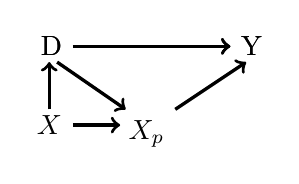
\begin{tikzpicture}
\draw[->,very thick] node [left] {D} (0,0)  -- (2,0) node [right] {Y} ;
\draw[->,very thick] node [left] {D} (0,0)  -- (2,0) node [right] {Y} ;
\draw[->,very thick]  (1.3,-.8) node [below left] {$X_p$}  -- (2.2,-.2) ;
\draw[<-,very thick] (.67,-.8) -- (-.2,-.2)  ;
\draw[->,very thick]  (0,-1) node [left] {$X$}  -- (.6,-1) ;	\draw[->,very thick]  (-.3,-.8)  -- (-.3,-0.2) ;	
\end{tikzpicture}
\end{center}
In practice, omitted variable bias concerns us most.\medskip

If we claim an absence of OVB, then we are saying that the regression is ok and has causal interpretation.\medskip

But the variables to control may not be observed and we look for a proxy $X_p$ of $X$ which might be affected by $D$\medskip

A delimma:
\begin{itemize}
\item If $X_p$ is not controlled, we have OVB.
\item If $X_p$ is controlled, we estimate partial effect netting out indirect effect through $X_p$
\end{itemize}
\end{frame}

\begin{frame}{Example of proxy variable}
\begin{itemize}
\item $X$ is ability or quality of high school students
\item $D$ is a self-selected education program in the first year of high school
\item $X_p$ is a test score in the second year (post treatment)
\item $Y$ is the test score in the third year.
\end{itemize}

Controlling $X_p$ reduces the effect of $D$ on $Y$, but it is better to control for it:
\begin{itemize}
\item If the effect is not zero then the estimation is ``conservative'' and the true effect is larger.
\end{itemize}
\end{frame}


\begin{frame}{Summary}
We talked about selection bias and two methods to remove it.
\begin{itemize}
\item Randomization
\item CIA and selection on observables.
\end{itemize}\bigskip

In the next lectures we'll discuss how to remove selection bias when it is due to unobservables. \bigskip

Based on data and problem different method can be applied: 
\begin{itemize}
\item instrumental variable, panel data, difference-in-difference, matching, regression discontinuity, etc.
\end{itemize} 
\end{frame}


%\begin{frame}{References:}
%\bibliographystyle{apalike}
%\small
%\bibliography{references}
%\end{frame}

\end{document}
